\chapter{The Truck Backer-Upper}
% Authors: Xiao Jing,  Changgeng Zhao, 4/30/2019

In this chapter, we present the process of collecting the data, training an emulator, training the control neural net and setting the loss function. 
\section{Setup}
\begin{minted}{python}
from matplotlib.pylab import *
from matplotlib.patches import Rectangle
from matplotlib.collections import PatchCollection
from matplotlib.lines import Line2D
π = pi

# Set up the cab and trailer
class Truck:
    def __init__(self, display=False):

        self.W = 1  # car and trailer width, for drawing only
        self.L = 1 * self.W  # car length
        self.d = 4 * self.L  # d_1
        self.s = -0.1  # speed
        self.display = display
        
        self.box = [0, 40, -10, 10]
        if self.display:
            self.f = figure(figsize=(10, 5), num='The truck backer-upper', facecolor='none')
            self.ax = self.f.add_axes([0.01, 0.01, 0.98, 0.98], facecolor='black')
            self.patches = list()
            
            self.ax.axis('equal')
            b = self.box
            self.ax.axis([b[0] - 1, b[1], b[2], b[3]])
            self.ax.set_xticks([], []); self.ax.set_yticks([], [])
            self.ax.axhline(); self.ax.axvline()

        self.reset()
    
    def reset(self, ϕ=0):
        self.ϕ = ϕ  # car initial steering angle
        
        # self.θ0 = deg2rad(30)  # car initial direction
        # self.θ1 = deg2rad(-30)  # trailer initial direction
        # self.x, self.y = 20, -5  # initial car coordinates
        
        self.θ0 = random() * 2 * π  # 0 <= ϑ₀ < 2π
        self.θ1 = (random() - 0.5) * π / 2 + self.θ0  # -π/4 <= ϑ₁ - ϑ₀ < π/4
        self.x = (random() * .75 + 0.25) * self.box[1]
        self.y = (random() - 0.5) * (self.box[3] - self.box[2])
        
        # If poorly initialise, then re-initialise
        if not self.valid():
            self.reset(ϕ)
        
        # Draw, if display is True
        if self.display: self.draw()
    
    def step(self, ϕ=0, dt=1):
        
        # Check for illegal conditions
        if self.is_jackknifed():
            print('The truck is jackknifed!')
            return
        
        if self.is_offscreen():
            print('The car or trailer is off screen')
            return
        
        self.ϕ = ϕ
        x, y, W, L, d, s, θ0, θ1, ϕ = self._get_atributes()
        
        # Perform state update
        self.x += s * cos(θ0) * dt
        self.y += s * sin(θ0) * dt
        self.θ0 += s / L * tan(ϕ) * dt
        self.θ1 += s / d * sin(θ0 - θ1) * dt
        
        return (self.x, self.y, self.θ0, *self._traler_xy(), self.θ1)
    
    def _get_atributes(self):
        return (
            self.x, self.y, self.W, self.L, self.d, self.s,
            self.θ0, self.θ1, self.ϕ
        )
    
    def _traler_xy(self):
        x, y, W, L, d, s, θ0, θ1, ϕ = self._get_atributes()
        return x - d * cos(θ1), y - d * sin(θ1)
        
    def is_jackknifed(self):
        x, y, W, L, d, s, θ0, θ1, ϕ = self._get_atributes()
        return abs(θ0 - θ1) * 180 / π > 90
    
    def is_offscreen(self):
        x, y, W, L, d, s, θ0, θ1, ϕ = self._get_atributes()
        
        x1, y1 = x + 1.5 * L * cos(θ0), y + 1.5 * L * sin(θ0)
        x2, y2 = self._traler_xy()
        
        b = self.box
        return not (
            b[0] <= x1 <= b[1] and b[2] <= y1 <= b[3] and
            b[0] <= x2 <= b[1] and b[2] <= y2 <= b[3]
        )
        
    def valid(self):
        return not self.is_jackknifed() and not self.is_offscreen()
        
    def draw(self):
        if not self.display: return
        if self.patches: self.clear()
        self._draw_car()
        self._draw_trailer()
        self.f.canvas.draw()
            
    def clear(self):
        for p in self.patches:
            p.remove()
        self.patches = list()
        
    def _draw_car(self):
        x, y, W, L, d, s, θ0, θ1, ϕ = self._get_atributes()
        ax = self.ax
        
        x1, y1 = x + L / 2 * cos(θ0), y + L / 2 * sin(θ0)
        bar = Line2D((x, x1), (y, y1), lw=5, color='C2', alpha=0.8)
        ax.add_line(bar)

        car = Rectangle(
            (x1, y1 - W / 2), L, W, 0, color='C2', alpha=0.8, transform=
            matplotlib.transforms.Affine2D().rotate_deg_around(x1, y1, θ0 * 180 / π) +
            ax.transData
        )
        ax.add_patch(car)

        x2, y2 = x1 + L / 2 ** 0.5 * cos(θ0 + π / 4), y1 + L / 2 ** 0.5 * sin(θ0 + π / 4)
        left_wheel = Line2D(
            (x2 - L / 4 * cos(θ0 + ϕ), x2 + L / 4 * cos(θ0 + ϕ)),
            (y2 - L / 4 * sin(θ0 + ϕ), y2 + L / 4 * sin(θ0 + ϕ)),
            lw=3, color='C5', alpha=1)
        ax.add_line(left_wheel)

        x3, y3 = x1 + L / 2 ** 0.5 * cos(π / 4 - θ0), y1 - L / 2 ** 0.5 * sin(π / 4 - θ0)
        right_wheel = Line2D(
            (x3 - L / 4 * cos(θ0 + ϕ), x3 + L / 4 * cos(θ0 + ϕ)),
            (y3 - L / 4 * sin(θ0 + ϕ), y3 + L / 4 * sin(θ0 + ϕ)),
            lw=3, color='C5', alpha=1)
        ax.add_line(right_wheel)
        
        self.patches += [car, bar, left_wheel, right_wheel]
        
    def _draw_trailer(self):
        x, y, W, L, d, s, θ0, θ1, ϕ = self._get_atributes()
        ax = self.ax
            
        x, y = x - d * cos(θ1), y - d * sin(θ1) - W / 2
        trailer = Rectangle(
            (x, y), d, W, 0, color='C0', alpha=0.8, transform=
            matplotlib.transforms.Affine2D().rotate_deg_around(x, y + W/2, θ1 * 180 / π) +
            ax.transData
        )
        ax.add_patch(trailer)
        
        self.patches += [trailer]
\end{minted}
\begin{figure}[H]
    \centering
    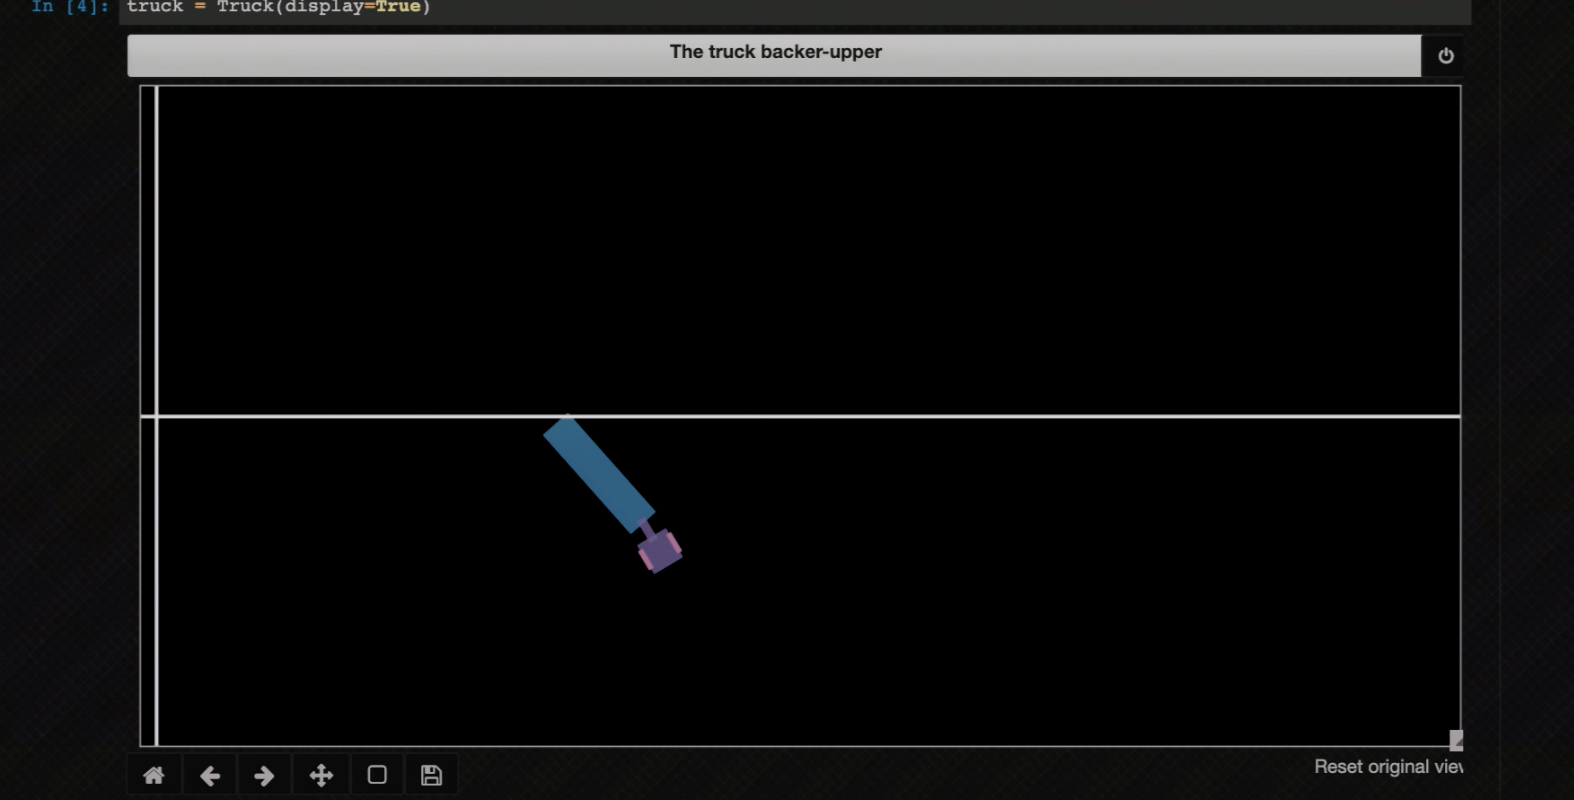
\includegraphics[width=0.7\textwidth]{labs/13/images/Screen Shot 2019-05-03 at 2.03.51 PM.png}
    \label{fig:state2}
    \caption{The interactive interface of the truck game. A player can set the angle of the front wheels
    of the truck at each step.}
\end{figure}
\\
\section{Collect Data}
\begin{minted}{python}
import torch
import torch.nn as nn
from torch.optim import SGD
from tqdm import tqdm

episodes = 10
data_set = list()
truck = Truck(); episodes = 10_000  # uncooment for creating the data set

for episode in tqdm(range(episodes)):
    
    truck.reset()
    states = list()
    
    while truck.valid():
        ϕ = (random() - 0.5) * π / 2
        states.append((ϕ, *truck.step(ϕ)))
        truck.draw()
    
    data_set.append(states)
\end{minted}

\section{Emulator Network and data preprocessing}
\begin{minted}{python}
state_size = 6
steering_size = 1
hidden_units_e = 45

emulator = nn.Sequential(
    nn.Linear(steering_size + state_size, hidden_units_e),
    nn.ReLU(),
    nn.Linear(hidden_units_e, state_size)
)

optimiser_e = SGD(emulator.parameters(), lr=0.05)
criterion = nn.MSELoss()

train_set = data_set[:8000]
test_set = data_set[8000:]

tensor_train_set = torch.cat([torch.Tensor(episode) for episode in train_set])
tensor_test_set = torch.cat([torch.Tensor(episode) for episode in test_set])

mean = tensor_train_set.mean(0)
std = tensor_train_set.std(0)
train_data = (tensor_train_set - mean) / std
test_data = (tensor_test_set - mean) / std


\end{minted}

\section{Train the emulator}
\begin{minted}{python}
i = 0
for episode in range(len(train_set)):
    episode_loss = 0
    for _ in range(len(train_set[episode]) - 1):
        ϕ_state = train_data[i]
        next_state_prediction = emulator(ϕ_state)
        
        next_state = train_data[i + 1, 1:]
        loss = criterion(next_state_prediction, next_state)
        episode_loss += loss.item()
        
        optimiser_e.zero_grad()
        loss.backward()
        optimiser_e.step()
        i += 1
    
    # Skip end, because there is no next_frame
    i += 1
    
    if (episode + 1) % 1000 == 0 or episode == 0:
        print(f'{episode + 1:4d} / {len(train_set)}, {episode_loss:.10f}')


\end{minted}

\section{Test the emulator}
\begin{minted}{python}
i = 0
total_loss = 0
with torch.no_grad():
    for episode in range(len(test_set)):
        for _ in range(len(test_set[episode]) - 1):
            ϕ_state = test_data[i]
            next_state_prediction = emulator(ϕ_state)

            next_state = train_data[i + 1, 1:]
            total_loss += criterion(next_state_prediction, next_state).item()

            i += 1

        # Skip end, because there is no next_frame
        i += 1
    
print(f'Test loss: {loss.item():.10f}')
\end{minted}